\chapter{Methodology}
As previously mentioned, both binary thresholding and deep learning feature map extraction as encoders have their downsides. Therefore, this thesis proposes to use a combination of both, a segmentation model which can extract classes into their respective SDRs. The video to be used is part of the VIRAT dataset.
\begin{figure}[H]
    \centering
    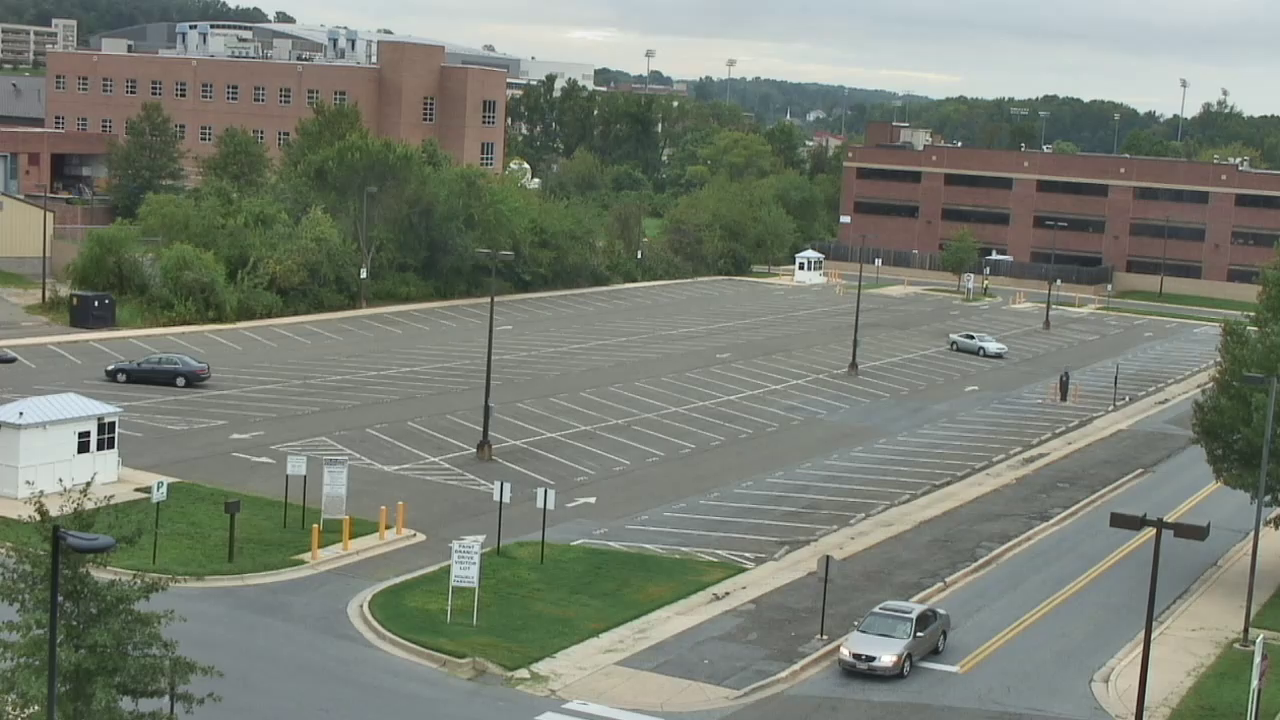
\includegraphics[width=.45\textwidth]{resources/methodology/original.png}\hfill
    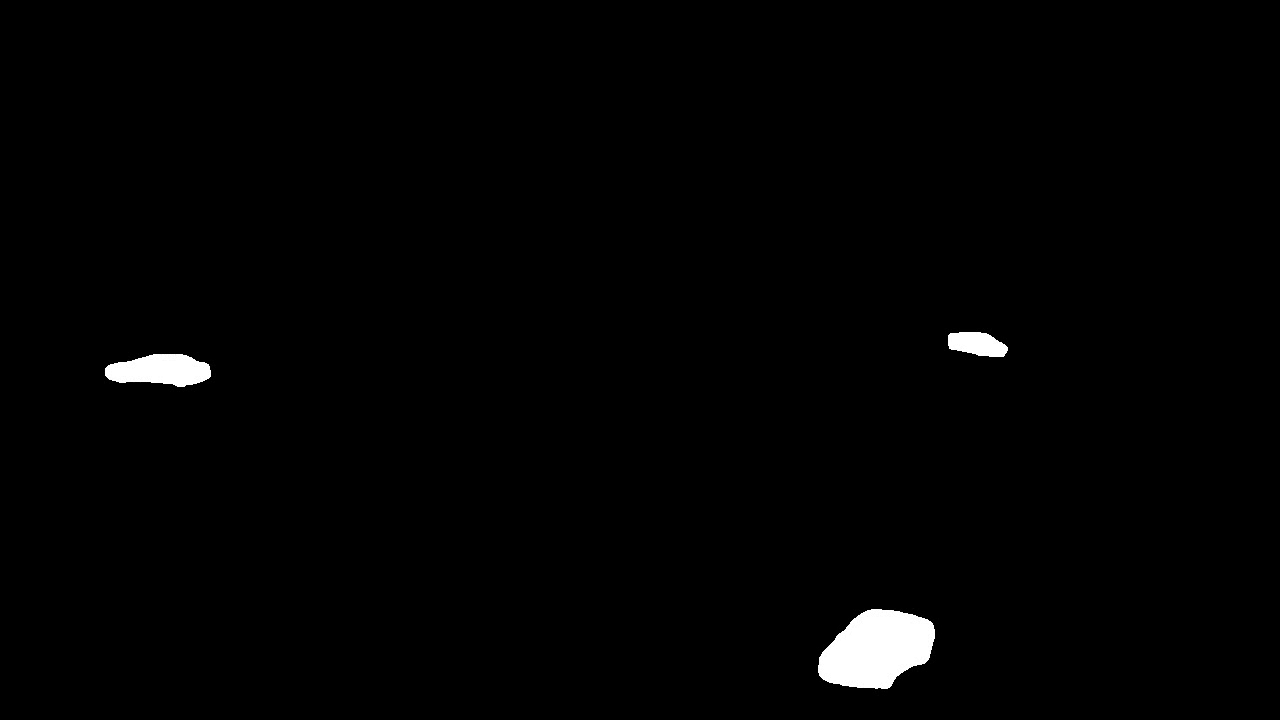
\includegraphics[width=.45\textwidth]{resources/methodology/car_segmentation.png}
    \caption{Segmentation result of cars}
    \label{fig:figure3}
\end{figure}
The idea is that the SP will learn to find an optimal general representation of cars. How general this representation is can be configured using the various parameters, but ideally they should be set so that different cars will be considered equal while trucks and motorcycles will be different. The task of the TM will then be to learn the common patterns that the cars exhibit, their speed, shape, and positioning will be taken into account. Finally, the learning will be set so that new patterns are learned quickly, but forgotten slowly. This will allow the system to quickly learn the norm, even if there is little activity, while still reacting to anomalies.\par
One issue that becomes evident is the lack of invariance. Because the TM is learning the global patterns, it learns that it is normal for cars to drive along the road but only in the context of there being cars parked in the parking lot. It is instead desired that the TM learns that it is normal for cars to drive along the road, regardless of whether there are cars in the parking lot. This thesis proposes a solution based on dividing the image into a grid, and have a separate SP and TM for each cell in the grid. The anomaly scores of all the cells are then aggregated into a single anomaly score.
\begin{figure}[H]
    \centering
    \includegraphics[width=0.7\textwidth]{example-image-a}
    \caption{The image divided into a grid.}
    \label{fig:grid}
\end{figure}
Another problem is that the previously mentioned rules for creating a good encoder may not be respected:
\begin{itemize}
    \item \textbf{Semantically similar data should result in SDRs with overlapping active bits}. In this case, a car at the one position will produce an SDR with a high amount of overlapping bits as another car at a similar position in the input image.
    \item \textbf{The same input should always produce the same SDR}. The segmentation produces a deterministic output given the same input.
    \item \textbf{The output must have the same dimensionality (total number of bits) for all inputs}. The segmentation output has a fixed dimensionality.
    \item \textbf{The output should have similar sparsity (similar amount of one-bits) for all inputs and have enough one-bits to handle noise and subsampling}. The segmentation model does not respect this. An example is that there can be no cars (zero active bits), one car ($n$ active bits), or two cars ($2n$ active bits).
\end{itemize}
The solution for the last rule is two-fold:
\begin{itemize}
    \item Pick a cell size so that the expected amount of active pixels when a cell contains car(s) is roughly the same.
    \item Create a pattern representing emptiness, where the number of active bits is similar to what can be expected on average when there are cars inside a cell.
\end{itemize}
\begin{figure}[H]
    \centering
    \includegraphics[width=0.7\textwidth]{example-image-b}
    \caption{Encoder output.}
    \label{fig:encoder_output}
\end{figure}

